% This is LLNCS.DEM the demonstration file of
% the LaTeX macro package from Springer-Verlag
% for Lecture Notes in Computer Science,
% version 2.4 for LaTeX2e as of 16. April 2010
%
\documentclass[a4paper]{llncs}
%

\usepackage{listings}
\usepackage{graphicx}
\usepackage{xspace}
\usepackage{pgf}
\usepackage[noend]{algpseudocode}
\usepackage{algorithm}

\usepackage{tikz}
\usetikzlibrary{arrows, automata, shapes}

\algrenewcommand\algorithmicrequire{\textbf{Precondition:}}
\algrenewcommand\algorithmicensure{\textbf{Postcondition:}}


\newcommand{\newC}{C$^-$\xspace}
\newcommand*\Let[2]{\State #1 $\gets$ #2}

\newcommand{\bv}[2]{\mathcal{BV}(#1, #2)}

%\usepackage{makeidx}  % allows for indexgeneration
%
\title{Fully Automatic Loop-free Program Synthesis by Bounded Model Checking}
\author{Daniel Kroening \and Matt Lewis}
\institute{University of Oxford}

\newenvironment{keywords}{
       \list{}{\advance\topsep by0.35cm\relax\small
       \leftmargin=0cm
       \labelwidth=0.35cm
       \listparindent=0.35cm
       \itemindent\listparindent
       \rightmargin\leftmargin}\item[\hskip\labelsep
                                     \bfseries Keywords:]}
     {\endlist}

\makeatletter
\pgfdeclareshape{datastore}{
  \inheritsavedanchors[from=rectangle]
  \inheritanchorborder[from=rectangle]
  \inheritanchor[from=rectangle]{center}
  \inheritanchor[from=rectangle]{base}
  \inheritanchor[from=rectangle]{north}
  \inheritanchor[from=rectangle]{north east}
  \inheritanchor[from=rectangle]{east}
  \inheritanchor[from=rectangle]{south east}
  \inheritanchor[from=rectangle]{south}
  \inheritanchor[from=rectangle]{south west}
  \inheritanchor[from=rectangle]{west}
  \inheritanchor[from=rectangle]{north west}
  \backgroundpath{
    %  store lower right in xa/ya and upper right in xb/yb
    \southwest \pgf@xa=\pgf@x \pgf@ya=\pgf@y
    \northeast \pgf@xb=\pgf@x \pgf@yb=\pgf@y
    \pgfpathmoveto{\pgfpoint{\pgf@xa}{\pgf@ya}}
    \pgfpathlineto{\pgfpoint{\pgf@xb}{\pgf@ya}}
    \pgfpathmoveto{\pgfpoint{\pgf@xa}{\pgf@yb}}
    \pgfpathlineto{\pgfpoint{\pgf@xb}{\pgf@yb}}
 }
}
\makeatother



\begin{document}
%
\maketitle
%
\pagestyle{headings}  % switches on printing of running heads

\begin{abstract}

We present a simple-yet-effective method for synthesizing loop-free programs
from specifications, using a novel combination of Bounded Model Checking and
explicit-state Model Checking.  The user provides a specification in plain
C, after which the synthesis process is fully automatic.

We demonstrate the effectiveness of our method by synthesizing several subtle
programs acting on machine integers, and a selection of floating-point programs.
\end{abstract}


\begin{keywords}
 Program synthesis, bitvectors, bounded model checking, CBMC,
 floating point.
\end{keywords}

\section{Introduction}

Program synthesis is the mechanized construction of software that provably
satisfies a given specification.  Synthesis tools promise to relieve the
programmer from thinking about \emph{how} the problem is to be solved;
instead, the programmer only provides a compact description of \emph{what}
is to be achieved.  Foundational research in this area has been
exceptionally fruitful, beginning with Alonzo Church's work on the
\emph{Circuit Synthesis Problem} in the sixties~\cite{church-synth}.

In this paper, we present a new method that brings the promise of
automating programming closer to application.  We make pragmatic
restrictions of the general synthesis problem in order to arrive at an
effective solution.  To this end, we focus on the problem of synthesizing
loop-free programs over machine integers and floating-point numbers from a
specification given as program fragment.  Our exploration of the program
space ensures that our programs are minimal in size.

Our work represents a substantial refinement of {\sc brahma}~\cite{brahma},
which is the closest work to ours.  {\sc Brahma} also focuses on
synthesizing loop-free machine-integer programs.  In~\cite{brahma}, the
authors characterise the program synthesis problem as a second-order
$\exists \forall$ formula and use a variation of the CEGIS algorithm,
introduced in~\cite{lezama-thesis}, for solving
these formulae.  This algorithm reduces the satisfiability of the $\exists
\forall$ formula to the satisfiability of several first-order formulae, each
of which can be decided using an off-the-shelf SMT solver.  {\sc Brahma}
takes as input a specification (given as an SMT formula) and a library of
components (one component is more or less a single machine instruction).  It
then finds a permutation of the component library that satisfies the
specification.  This permutation is the final synthesised program.  In the
event that the library does not contain enough components to synthesise a
correct program, the user is told that the library is too small and is
must add more components until the synthesis succeeds.  Each round of
synthesis amounts to solving an $\exists \forall$ formula that is quadratic
in the size of the component library.

We require the user to supply a program specification written in C, but then
ask nothing more of her.  We parameterise the space of programs in such a way
that it can be explored automatically, rather than asking a human for hints.
Our program encoding allows generates an $\exists
\forall$ formula that is \emph{linear} in the length of the shortest program
satisfying the user's specification, which we then check for satisfiability
using the CEGIS algorithm.  In contrast, the program generated by {\sc
brahma} can be no longer than the size of the library, as the synthesis
outcome is a permutation of the component library.  Our synthesis
formulae are therefore asymptotically smaller than {\sc brahma}'s.

\paragraph{Related Work}

Another successful approach to program synthesis has been \emph{program
sketching}, in particular the {\sc sketch} tool~\cite{lezama-thesis,sketch}.  This method
requires the programmer to provide a \emph{program sketch}, written in a
C-like language, together with either a specification (written in the same
language) or a suite of unit tests.  The sketch is a skeleton program which
contains much of the high-level structure of the final program, but with
several ``holes'', which {\sc sketch} fills in to meet the specification,
again using the CEGIS algorithm.

Program synthesis is closely related to
superoptimisation~\cite{superoptimisation}, which is the problem of taking a
segment of code, usually written in C, and finding a minimal program which
has the same functionality.  The {\sc aha}~\cite{aha} tool and the GNU
superoptimiser~\cite{gnu-superoptimiser} both perform superoptimisation of C
programs, both by enumerating possible programs and testing them on suitable
inputs.  This search can be compiled down to native code using an optimising
compiler, so for short programs the method is extremely fast.  However, this
method is impractical for synthesising longer programs because of the
exponential blowup of the search space.  We incorporate the core idea of
this technique by using explicit-state model checking in parallel with
symbolic model checking.

\paragraph{Technical Contributions}
Our approach generates an $\exists \forall$ formula which is linear
in the size of the synthesised program.  This improves over the
encoding of~\cite{brahma}, which generates a $\exists \forall$ formula
that is quadratic in the size of the synthesised program.

We introduce a novel parameterisation of the programming language
used to express our synthesised programs.
This parameterisation allows us to efficiently explore the program space
without relying on human guidance and also ensures that our programs
are of minimal length.

Our tool is the first we are aware of that is able to effectively
synthesise floating point programs.  We demonstrate this by
synthesising {\sc Fast2Sum} using Knuth's {\sc 2Sum}~\cite{taocp2} as
a specification.

\paragraph{Outline} We give details of our new algorithm in
Sec.~\ref{sec:algorithm}.  We use a fragment of the C programming language
as our underlying logic, which is elaborated in Sec.~\ref{sec:logic}. We
summarize the results of our experiments in Sec.~\ref{sec:experiments}.

\section{The Basic Synthesis Algorithm}
\label{sec:algorithm}

\subsection{The Synthesis Formula}
\label{sec:abstract-formula}

Our task is to find a program which satisfies some specification.  We can formalize this
notion as follows: fix an input set $I$ and an output set $O$.  Specifications $\sigma$
relate inputs and outputs, and programs $P$ map an input to an output:
%
$$ \sigma \subseteq I \times O $$
$$ P : I \rightarrow O$$

The synthesis problem is then to determine the validity of the following
second-order formula, and if so, to find a suitable witness program $P$:
%
$$\exists P .\, \forall x \in I.\, \sigma(x, P(x))$$

Depending on the logic needed to express this formula the synthesis problem
may be decidable, semi-decidable or undecidable.  For many interesting
logics, checking the validity of a second-order formula is undecidable. 
Even for logics in which the problem is decidable, the quantifier
alternation means that we may not have an efficient decision procedure for
the formula above, although efficient methods may exist for solving problems
with only one quantifier.  In particular, in the case of propositional
satisfiability, we have SAT solvers which are efficient-in-practice at
solving queries with a single quantifier.  The corresponding problem with
one level of quantifier alternation (2-QBF) is complete for $NP^{NP}$, and
current 2-QBF solvers are much less efficient in practice than SAT solvers.

\subsection{CEGIS}

When the quantifier free first-order fragment of the logic is efficiently decidable and
$P$ can be expressed as a quantifier free term of the logic, we can use
Counterexample Guided Inductive Synthesis (CEGIS)~\cite{lezama-thesis,sketch} to
check the validity of the synthesis formula.  The core of the CEGIS algorithm is
a refinement loop to check the
validity of the synthesis formula as shown in Fig.~\ref{fig:abstract-refinement} and
Algorithm~\ref{fig:abstract-refinement-code}.  The algorithm is divided into two
components: {\sc synth} and {\sc verif}.  We track a finite (small) subset of test inputs
and {\sc synth} synthesises a candidate program that is correct on just those tests.
{\sc Verif} then tries to verify the candidate program by searching for an input on
which the candidate program does not satisfy the specification.  If no such input
can be found, the candidate program is correct.  Otherwise, the new input is added
to the set of inputs we must check in {\sc synth}.  If the input set is finite, this
procedure is guaranteed to terminate.

\begin{figure}
 \centering
 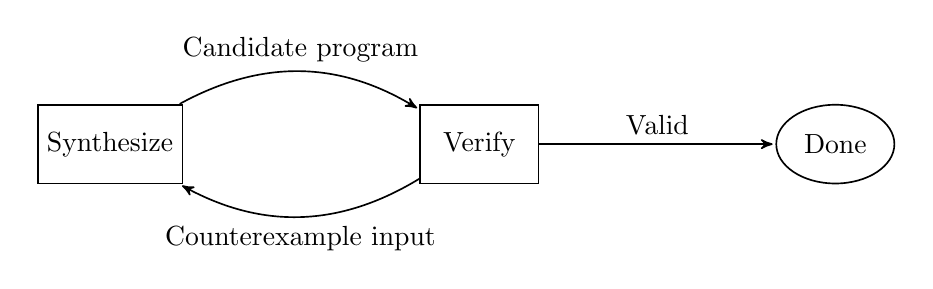
\begin{tikzpicture}[->,>=stealth',shorten >=1pt,auto,
 semithick, initial text=]

  \matrix[nodes={draw, fill=none, scale=1, shape=rectangle, minimum height=1cm, minimum width=1.5cm},
          row sep=2cm, column sep=3cm] {
   \node (synth) {Synthesize};
   &
   \node (verif) {Verify}; %\\
   %\node[draw=none] {};
   &
   \node[ellipse] (done) {Done}; \\
  };

   \path
    (synth) edge [bend left] node {Candidate program} (verif)
    (verif) edge [bend left] node {Counterexample input} (synth)
    (verif) edge node {Valid} (done);
 \end{tikzpicture}
 
 \caption{Abstract synthesis refinement loop
 \label{fig:abstract-refinement}}
\end{figure}

\begin{algorithm}
 \caption{Abstract refinement algorithm
 \label{fig:abstract-refinement-code}}
 

 \begin{algorithmic}[1]
\Statex
\Function{synth}{inputs}
  \Let{$(i_1, \ldots, i_N)$}{inputs}
  \Let{query}{$\exists P . \sigma(i_1, P(i_1)) \land \ldots \land \sigma(i_N, P(i_N))$}
  \Let{result}{decide(query)}
  \If{result.satisfiable}
    \State \Return{result.model}
  \Else
    \State \Return{unsatisfiable}
  \EndIf
\EndFunction
\Statex
\Function{verif}{P}
  \Let{query}{$\exists x . \lnot \sigma(x, P(x))$}
  \Let{result}{decide(query)}
  \If{result.satisfiable}
    \State \Return{result.model}
  \Else
    \State \Return{valid}
  \EndIf
\EndFunction
\Statex
\Function{refinement loop}{}
  \Let{inputs}{$\emptyset$}
  \Loop
    \Let{candidate}{synth(inputs)}
    \If{candidate = unsatisfiable}
      \State \Return{unsatisfiable}
    \EndIf
    \Let{res}{verif(candidate)}
    \If{res = valid}
      \State \Return{candidate}
    \Else
      \Let{inputs}{inputs $\cup$ res}
    \EndIf
  \EndLoop
\EndFunction
 \end{algorithmic}
\end{algorithm}


\section{\newC}
\label{sec:logic}

We use a fragment of C as our underlying logic.  We will refer to this fragment
as \newC.  The characteristic property of \newC is that safety can be decided for
\newC programs using a single query to a Bounded Model Checker.  A \newC program is
just a C program with the following syntactic restrictions:

\begin{itemize}
 \item All loops in the program must have a constant bound.
 \item All recursion in the program must be limited to a constant depth.
 \item All arrays must be statically allocated (i.e. not using \texttt{malloc}),
 and be of constant size.
\end{itemize}

Additionally, \newC programs may use nondeterministic values, assumptions
and arbitrary-width types.

\begin{figure}
\begin{minipage}[scale=0.8]{0.45\linewidth}
 \begin{lstlisting}[language=c]
int count_bits(int x) {
  int i, ret;
  
  ret = 0;
  
  for (i = 0; i < 32; i++)
    if (x & (1 << i))
      ret++;
  
  return ret;
}
 \end{lstlisting}
\end{minipage}
\begin{minipage}{0.54\linewidth}
 \begin{lstlisting}[language=C]
int common_factor(int A[10]) {
  int factor = nondet();
  int i;

  for (i = 0; i < 10; i++)
    assume((A[i] % factor) == 0);

  assume(factor > 1);
  return factor;
}

 \end{lstlisting}
\end{minipage}

 \caption{Two \newC programs}
 \label{fig:c-}

\end{figure}

Since each loop is bounded by a constant, and each recursive function call is
limited to a constant depth, a \newC program necessarily terminates and in
fact does so in $O(1)$ time.  If we call the largest loop bound~$k$, then
a Bounded Model Checker with an unrolling bound of $k$ will be a complete
decision procedure for the safety of the program.  For a \newC program of
size $l$ and with largest loop bound~$k$, a Bounded Model Checker will
create a SAT problem of size $O(lk)$.  Conversely, a SAT problem
of size $s$ can be converted trivially into a loop-free \newC program
of size $O(s)$.  The safety problem for \newC is therefore NP-complete,
which means it can be decided fairly efficiently for many practical
instances.

\subsection{Why use \newC instead of SAT?}
To misquote David Wheeler: ``all problems in computer science can be solved by
another level of abstraction''~\cite{beautiful-code}.  \newC serves as
an abstraction of SAT.  We can think of SAT as an assembly language and
{\sc cbmc} as a compiler for \newC to this assembly language.  The benefits
of using \newC as our logic rather than SAT are very similar to the benefits of
writing code in a high level language rather than assembly language.
Some of the more significant advantages are:

\begin{itemize}
 \item The code is more readable and easier to debug.
 \item The code is much more concise.
 \item We can take advantage of new optimisations, different model
 checkers and different back-ends (SAT, SMT, ACDCL, etc.) for free.
\end{itemize}

To illustrate some of these points, we were able to implement a first
version of {\sc kalashnikov} in around 150 lines of code, which took around
two hours to write.  The resulting code was easy to modify, optimise and
debug.  The current version, which includes support for floating-point
arithmetic, several optimisations and two model checking algorithms, is
still less than 1200 lines of code (600 lines of \newC and 600 lines of
Python).

Another benefit of using \newC as our logic is that it would be easy to
automatically extract specifications from C programs, which would be
useful in the context of superoptimisation.  This is because \newC is
a relatively large fragment of C, so we anticipate that many interesting
sections of real code will already be~\newC.


\section{The Concrete Algorithm for Bitvector Programs}

One area in which program synthesis can shine is in producing very small,
intricate programs that manipulate bitvectors.  An example of such a program
is shown in Fig.~\ref{fig:bitvector-program}.  This program takes a machine word
as input and clears every bit except for the least significant bit that was set.
Even though this program is extremely short, it is fairly difficult for a human
to see what it does.  It is even more difficult for a human to come up with such
minimal code -- a natural solution for this problem might be to use a loop which
iterates over all of the bits in the word.  The program is so concise because it
takes advantage of the low-level details of the machine, such as the fact that
signed integers are stored in two's complement form.

\begin{figure}
\centering
\begin{minipage}{0.45\linewidth}
 \begin{lstlisting}[language=C]
int isolate_lsb(int x) {
  return x & -x;
}
 \end{lstlisting}
\end{minipage}
\begin{minipage}{0.45\linewidth}
 
Example:

\hrule

\begin{tabular}{llcccccccc}
 x       & = & 1 & 0 & 1 & 1 & 1 & 0 & 1 & 0 \\
 -x      & = & 0 & 1 & 0 & 0 & 0 & 1 & 1 & 0 \\
 x \& -x & = & 0 & 0 & 0 & 0 & 0 & 0 & 1 & 0
\end{tabular}
\end{minipage}


 \caption{A tricky bitvector program}
  \label{fig:bitvector-program}
\end{figure}


To synthesise tricky bitvector programs like this, it is natural for us to
work in the logic of quantifier-free propositional formulae and to use a
propositional SAT or SMT-$\mathcal{BV}$ solver as the decision procedure. 
However, we propose a slightly different tack, which is to use \newC as
our underlying logic.

To instantiate the abstract synthesis algorithm in \newC we must express $I, O,
\sigma$ and $P$ in \newC, then ensure that we can express the validity of the
synthesis formula as a safety property of the resulting \newC program.

Our encoding is the following:
%
\begin{itemize}
 \item $I$ is the type \verb|int[N]|.
 \item $O$ is the type \verb|int[M]|.
 \item $\sigma$ is a function with signature
 \verb|int check(int in[N], int out[M])|. This function is the only component supplied
 by the user.
 \item $P$ is written in a simple RISC-like language $\mathcal{L}$.  Programs in $\mathcal{L}$
 have the type \verb|prog_t|.
 \item We supply an interpreter for $\mathcal{L}$ which is written in \newC.  The signature
 of this interpreter is \\
 \verb|void exec(prog_t p, int in[N], int out[M])|.
\end{itemize}

\begin{figure}
\begin{center}
\setlength{\tabcolsep}{16pt}
Integer arithmetic instructions:

\begin{tabular}{llll}
 \verb|add a b| & \verb|sub a b| & \verb|mul a b| & \verb|div a b| \\
 \verb|neg a| & & &
\end{tabular}

\medskip

Bitwise logical and shift instructions:

\begin{tabular}{llll}
 \verb|and  a b| & \verb|or a b| & \verb|xor a b| & \verb|ashr a b| \\
 \verb|lshr a b| & \verb|not  a| & &
\end{tabular}

\medskip

Unsigned and signed comparison instructions:

\begin{tabular}{llll}
 \verb|le  a b| & \verb|lt  a b| & \verb|sle  a b| & \verb|slt a b|
\end{tabular}
\end{center}

 \caption{The language $\mathcal{L}$}
 \label{fig:l-language}

\end{figure}

We must now express the {\sc synth} and {\sc verif} formulae as safety properties
of \newC programs, which is shown in Fig.~\ref{fig:c-synthverif}.

\begin{figure}
\centering
\begin{minipage}{0.45\textwidth}
\begin{lstlisting}[language=C++]
void synth() {
  prog_t p = nondet();
  int in[N], out[M];
  
  in = test1;
  exec(p, in, out);
  assume(check(in, out));
  
  ...
  
  in = testN;
  exec(p, in, out);
  assume(check(in, out));
  
  assert(false);
}
\end{lstlisting}
\end{minipage}
\begin{minipage}{0.45\textwidth}
\begin{lstlisting}[language=C]
void verif(prog_t p) {
  int in[N] = nondet();
  int out[M];

  exec(p, in, out);
  assert(check(in, out));
}
\end{lstlisting}
\end{minipage}

 \caption{The {\sc synth} and {\sc verif} formulae expressed as a \newC program}
 \label{fig:c-synthverif}
\end{figure}

In order to determine the validity of the {\sc synth} formula, we can now
check the {\sc synth} program for safety.  The {\sc synth} program is a
\newC program, which means we can check its safety by invoking a Bounded
Model Checker, such as {\sc cbmc}.

In some cases, it is faster to use an explicit-state model checker rather
than a Bounded Model Checker.  This is particularly true when we are checking
the {\sc verif} formula, where we have observed that incorrect programs tend
to be incorrect on a large fraction of the input space.  Counterexamples
are then very easy to find by explicit enumeration of a few inputs.
Since \newC is a fragment of C, we can generate an explicit-state
model checker using the same source files that we pass to {\sc cbmc}
and adding a small function which enumerates possible inputs.
We can run the explicit-state model checker
in parallel with {\sc cbmc} and take the answer of whichever happens
to terminate first, stopping the other process.  This procedure is
depicted for {\sc synth} in Fig.~\ref{fig:synth-dfd}, and is similar for {\sc verif}.

\begin{figure}
\begin{center}
\tikzstyle{file}=[draw, text width=7.0em, text centered,
  minimum height=1.5em]
\tikzstyle{process} = [draw, minimum height=3em, circle]
\tikzstyle{line} = [draw, color=black, -latex']


\begin{tikzpicture}[font=\sffamily]

\node [file] (synth) {\sc synth.c};
\path (synth.south)+(0.0, -0.5) node [file] (tests) {\sc tests.c};
\path (tests.south)+(0.0, -0.5) node [file] (interpreter) {\sc interpreter.c};
\path (interpreter.south)+(0.0, -0.5) node [file] (spec) {\sc spec.c};

\path (tests.east)+(2.0, -0.25) node [process] (merged) {merge};

\path (merged.east)+(2.0, 1.0) node [process] (cbmc) {\sc cbmc};
\path (merged.east)+(2.0, -1.0) node [process] (gcc) {\sc gcc};

\path (cbmc.east)+(2.5, -1.0) node [file] (out) {candidate program};

\path [line] (synth) -- (merged);
\path [line] (tests) -- (merged);
\path [line] (interpreter) -- (merged);
\path [line] (spec) -- (merged);

\path [line] (merged) -- (cbmc);
\path [line] (merged) -- (gcc);

\path [line] (cbmc) -- (out);
\path [line] (gcc) -- (out);

\end{tikzpicture}
\end{center}

\caption{Schematic diagram of {\sc synth}}
\label{fig:synth-dfd}
\end{figure}

\subsection{Implementation Issues}
For performance reasons, we found that adding extra constraints on the
shape of the synthesised programs sped up synthesis.  The extra constraints
fell into two categories: eliminating nops and instruction-level symmetry reduction.

\subsubsection{Remove nops}
Many instructions in $\mathcal{L}$ are nops that do not doing anything.
For example the instruction \verb|add x 0| does nothing.  Such instructions
can be removed from any program they appear in to leave a semantically
equivalent, but shorter, program.  We can therefore be sure that nops
will never appear in any minimal program.  By adding constraints saying that
each instruction is not a nop, we can help the underlying SAT solver's
search, which reduces the runtime of the overall procedure.

\subsubsection{Symmetry Reduction}
There are many instructions that are equivalent to each other.  For example,
\verb|add x y| is equivalent to \verb|add y x| -- any program containing
one instruction could have it replaced by the other instruction and
keep the same semantics.  We choose a single canonical instruction to
represent all instructions in a particular equivalence class, then add
constraints saying that no non-canonical instructions appear in the program.

Our rules for excluding non-canonical instructions are:

\begin{itemize}
 \item For commutative operations, the first operand is smaller than the second.
 \item For unary operations, the second (unused) operand is always 0.
 \item No instruction may have two constant operands.
 \item All constants in the constant table are distinct.
\end{itemize}

As with the nop constraints, these additional constraints do increase the
size of the resulting SAT instance, but this still ends up as a win in
terms of runtime.


\section{Parameterising the Program Space}
In order to search the space of candidate programs, we parameterise
the language~$\mathcal{L}$, creating a lattice of progressively
more expressive languages.  We start by attempting to synthesise
a program at the lowest point on this lattice and increase the
parameters of~$\mathcal{L}$ until we reach a point at which
the synthesis succeeds.

As well as giving us an automatic search procedure, this paramterisation
greatly increases the efficiency of our system since languages
low down the lattice are very easy to decide safety for.  If a program
can be synthesised in a low-complexity language, the whole procedure
finishes much faster than if synthesis had been attempted in a
high-complexity language.  Our paramterisation is constructed
in such a way that the programs we synthesise are guaranteed to be
minimal in length.

\subsection{Program Length: $l$}
The first paramter we introduce is program length, denoted by $l$.
At each iteration we synthesise programs of length exactly $l$.
We start with $l = 1$ and increment $l$ by $1$ when we have determined
that no program of length $l$ can satisfy the specifcation.  When we do
successfully synthesise a program, we are guaranteed that it
is of minimal length since we have previously established that no
correct program of smaller length exists.


\subsection{Word Width: $w$}
An $\mathcal{L}$-program runs on a virtual machine (the $\mathcal{L}$-machine) that
has its own set of paramters.  The only relevant parameter is
the \emph{word width} of the $\mathcal{L}$-machine, that is, the number of bits
in each internal register and immediate constant.  This parameter is denoted by
$w$.  The size of the final SAT problem generated by {\sc cbmc} scales
approximately linearly with $w$, since each intermediate C variable corresponds
to $w$ propositional variables.

It is often the case that a program which satisfies the specification
on an $\mathcal{L}$-machine with $w = k$ will continue to satisfy the
specification when run on a machine with $w > k$.  For example, the program
in Fig.~\ref{fig:bitvector-program} isolates the least-significant bit of a word.
This is true irrespective of the word size of the machine it is run on -- it will
isolate the least-significant bit of an 8-bit word just as well as it will a
32-bit word.  An often successful strategy is to synthesise a program for an
$\mathcal{L}$-machine with a small word size and then to check whether the
same program is correct when run on an $\mathcal{L}$-machine with a
full-sized word.

The only wrinkle here is that we will sometimes synthesise a program containing
constants.  If we have synthesised a program for with $w=k$,
the constants in the program will be $k$-bits wide.  To generalize the program
to an $n$-bit machine (with $n > k$), we need some way of deriving $n$-bit-wide
numbers from $k$-bit ones.  We have several strategies for this and
just try each in turn.  The strategies are shown in Fig.~\ref{fig:generalize},
where $\mathcal{BV}(v, n)$ denotes an $n$-bit wide bitvector holding the value $v$
and $b \cdotp c$ means the concatenation of bitvectors $b$ and $c$.

\begin{figure}

\begin{eqnarray*}
 \bv{m}{m} & \rightarrow & \bv{n}{n} \\
 \bv{m-1}{m} & \rightarrow & \bv{n-1}{n} \\
 \bv{m+1}{m} & \rightarrow & \bv{n+1}{n} \\
 \bv{x}{m} & \rightarrow & \bv{x}{n} \\
 \bv{x}{m} & \rightarrow & \bv{x}{m} \cdotp \bv{0}{n - m} \\
 \bv{x}{m} & \rightarrow & \underbrace{\bv{x}{m} \cdotp \ldots \cdotp \bv{x}{m}}_{\frac{n}{m} \mathrm{ times}}
\end{eqnarray*}

\caption{Rules for generalizing 
an $m$-bit wide number to an $n$-bit wide one
 \label{fig:generalize}}
\end{figure}

Sometimes a program will be correct for some particular word width $w$, but is
not correct for $w' > w$ even if the constants are replaced with appropriate ones.
When this happens we are forced to increase $w$ and continue synthesising.

\subsection{Number of Constants: $c$}
Instructions in $\mathcal{L}$ take either one or two operands.
Since any instruction whose operands are all constants can always be
eliminated (since its result is a constant), we know that a loop-free program
of minimal length will not contain any instructions with two constant
operands.  Therefore the number of constants which can appear in
a minimal program of length $l$ is at most $2l$.  By minimising the number
of constants appearing in a program, we are able to use a particularly
efficient program encoding that speeds up the synthesis procedure
substantially.  The number of constants used in a program is the parameter $c$.

$\mathcal{L}$ is an SSA, three address instruction set\footnote{
We experimented with implementing $\mathcal{L}$ as a stack machine, expecting
the programs to be smaller and synthesis to be faster as a result.  We saw
the opposite effect -- the more complex interpreter led to much slower synthesis.
}.  Destination registers
are implicit and a fresh register exists for each instruction to write its
output to.  A na\"{\i}ve way to encode $\mathcal{L}$ instructions is to have an
opcode and two operands, where each operand is either a register (i.e., a program argument
or the result of a previous instruction), or an immediate constant.

In this encoding, each opcode requires $\lceil \log_2 I \rceil$ bits to encode, where $I$ is the number
of instruction types in $\mathcal{L}$.  Each operand can be encoded using
$\log_2 w$ bits, where $w$ is the $\mathcal{L}$-machine word, plus one
bit to specify whether the operand is a register name or an immediate constant.
One instruction can therefore be encoded using $\lceil \log_2 I \rceil + 2w + 2$ bits.
For an $n$ instruction program, we need $$\lceil n \log_2 I \rceil + 2nw + 2n$$ bits to encode
the entire program.

If we instead limit the number of constants that can appear in the program,
our operands can be encoded using fewer bits.  For an $n$ instruction program
using $c$ constants and taking $a$ arguments as inputs, each operand can refer
to a program argument, the result of a previous instruction or a constant.
This can be encoded using $\lceil \log_2 (c+a+n-1) \rceil$ bits, which means each instruction
can be encoded in $\lceil \log_2 I \rceil + \lceil \log_2 (c + a + n - 1) \rceil$ and the full program
needs $$\lceil n \log_2 I \rceil + \lceil n \log_2 (c + a + n - 1) \rceil + cw$$ bits to encode.

To give an example, $\mathcal{L}$ has 15 instruction types, so each opcode is 4 bits.
For a 10 instruction program over 1 argument, using 2 constants on a 32-bit word
machine the first encoding requires $10 * (4 + 32 + 1 + 32 + 1) = 700$ bits.
Using the second encoding, each operand can be represented using
$\log_2 (2 + 1 + 10 - 1) = 4$ bits, and the entire program requires 184 bits.
This is a substantial reduction in size and when the required program requires
few constants this can lead to a very significant speed up.

As with program length we can progressively increase the number of constants in
our program.  We start by trying to synthesise a program with no constants, then
if that fails we try to synthesise using one constant and so on until we reach
$c = l$.

\subsection{Searching the Program Space}
The key to our automation approach is to come up with a sensible way in which to
adjust the $\mathcal{L}$-parameters in order to cover all possible programs.
After each round of {\sc synth}, we may need to adjust the parameters.  The
logic for these adjustments is shown as a tree in Fig~\ref{fig:paramsflow}.


\begin{figure}
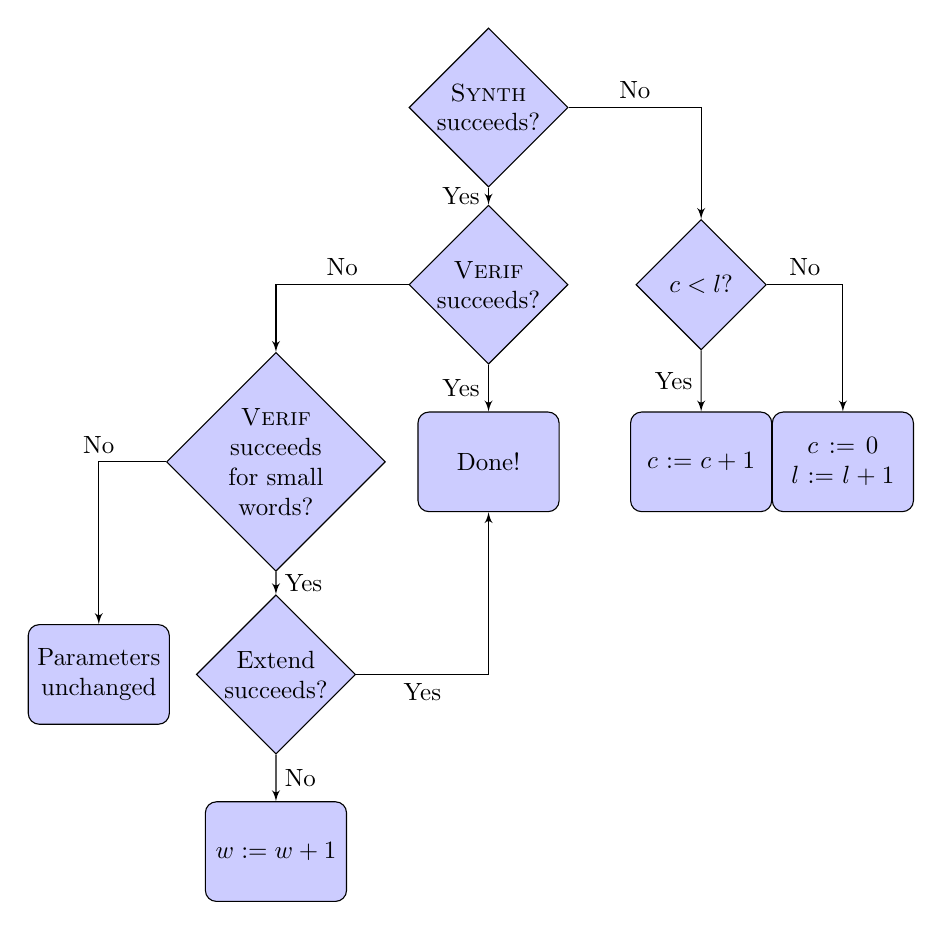
\begin{tikzpicture}[scale=0.9, transform shape, node distance=2cm, auto]
\tikzstyle{decision} = [diamond, draw, fill=blue!20, 
    text width=4.5em, text badly centered, node distance=3cm, inner sep=0pt]
\tikzstyle{block} = [rectangle, draw, fill=blue!20, 
    text width=5em, text centered, rounded corners, minimum height=4em]
\tikzstyle{line} = [draw, -latex']
\tikzstyle{cloud} = [draw, ellipse,fill=red!20, node distance=3cm,
    minimum height=2em]

 \node [decision] (synthsucc) {{\sc Synth} succeeds?};

 \node [decision, below of=synthsucc, node distance=2.5cm] (verif) {{\sc Verif} succeeds?};
 \node [decision, right of=verif] (ck) {$c < l$?};

 \node [block, below of=verif, node distance=2.5cm]   (done) {Done!};
 \node [decision, left of=done] (verifw) {{\sc Verif} succeeds for small words?};

 \node [block, below of=ck, node distance=2.5cm] (incc) {$c := c+1$};
 \node [block, right of=incc, node distance=2cm] (incl) {$c := 0$\\ $l := l+1$};

 \node [decision, below of=verifw, node distance=3cm] (gen) {Extend succeeds?};
 \node [block, left of=gen, node distance=2.5cm] (iterate) {Parameters unchanged};

 \node [block, below of=gen, node distance=2.5cm] (incw) {$w := w+1$};

 \path [line] (synthsucc) -- node [left] {Yes} (verif);
 \path [line] (synthsucc) -| node [above, near start] {No} (ck);

 \path [line] (verif) -- node [left] {Yes} (done);
 \path [line] (verif) -| node [above, near start] {No} (verifw);

 \path [line] (ck) -- node [left] {Yes} (incc);
 \path [line] (ck) -| node  [above, near start]  {No} (incl);

 \path [line] (verifw) -- node [right] {Yes} (gen);
 \path [line] (verifw) -| node [above] {No} (iterate);
 
 \path [line] (gen) -| node [below, near start] {Yes} (done);
 \path [line] (gen) -- node [right] {No} (incw);

 %\path [dotted, line] (iterate.west) |- (synthsucc);
\end{tikzpicture}

 \caption{Decision tree for increasing parameters of $\mathcal{L}$.}
 \label{fig:paramsflow}

\end{figure}

\begin{figure}
\begin{center}
\begin{minipage}[t]{0.45\linewidth}
\begin{algorithm}[H]
\caption{\sc 2Sum
 \label{alg:2sum}}
\begin{algorithmic}
\Let{$s$}{$a+b$}
\Let{$b'$}{$s - a$}
\Let{$a'$}{$s - b'$}
\Let{$\delta b$}{$b - b'$}
\Let{$\delta a$}{$a - a'$}
\Let{$t$}{$\delta a + \delta b$}
\Ensure{$a + b$ = $s + t$ exactly}
\end{algorithmic}
\end{algorithm}
\end{minipage}
\hfill
\begin{minipage}[t]{0.45\linewidth}
\begin{algorithm}[H]
\caption{\sc Fast2Sum
 \label{alg:fast2sum}}
\begin{algorithmic}
\Require{$a \ge b$}
\Let{$s$}{$a + b$}
\Let{$z$}{$s - a$}
\Let{$t$}{$b - z$}
\Ensure{$a + b$ = $s + t$ exactly}
\end{algorithmic}
\end{algorithm}
\end{minipage}
\end{center}

 
 \caption{The {\sc 2Sum} algorithm for correctly rounded floating point sums.}
  \label{fig:2sum}
\end{figure}


\section{Experimental Results}
\label{sec:experiments}
We implemented our synthesis procedure as the {\sc kalashnikov} tool.  The implementation consists
of around 600 lines of \newC and 600 lines of Python.  To evaluate the tool we used the 25 bitvector
programs from~\cite{brahma}.  The code we used to perform the experiments, along with the
benchmarks, is available at \texttt{http://www.cprover.org/kalashnikov}.  As a backend solver, we used
{\sc CBMC} at SVN revision r2777, using Glucose 2.2~\cite{glucose} as the SAT solver.
We performed our experiments on a 4-core, 3.07\,GHz Xeon X5667 with 50\,GB of RAM.

To give a reference point for the efficiency of our tool, we present the results given for {\sc brahma}
on the same benchmarks, as reported in~\cite{brahma}.  These experiments were performed an 8-core,
1.86\,GHz Xeon with 4\,GB of RAM, so the timings should be comparable to within a factor of 2 or so.

The results of our experiments are shown in Fig.~\ref{fig:results-table}.  On the problems for which
we are able to synthesise a program, we take a similar time to {\sc brahma}.  We are unable to synthesise
programs for 6 of the 25 problems that {\sc brahma} is able to solve.  We believe this to be a result of
the slight difference in the problems solved by {\sc kalashnikov} and {\sc brahma}.  We do not ask the
user for any information beyond the program specification, whereas {\sc brahma} asks for an extended
component library when synthesis with the standard library fails.  This extended library contains a
reasonable amount of information about the structure of the final program, which we believe makes
problems P19 to P25 tractable for {\sc brahma} but intractable for us.

To demonstrate the capabilities of \newC as an impementation language, we synthesise a
non-trivial floating point program.  For this we chose the classic {\sc 2Sum} algorithm for computing
exact sums of floating point numbers.  The original {\sc 2Sum} algorithm is shown in Alg.~\ref{alg:2sum}.
In the case that $a \ge b$, exact addition can be implemented in fewer instructions -- this is the
{\sc Fast2Sum} algorithm~\cite{fast2sum}.  We used {\sc 2sum} as our specification, and
added an assumption that $a \ge b$.  {\sc Kalashnikov} is able to synthesise and verify the
code for {\sc Fast2Sum} from this specification in 396.07\,s, which we believe to be the first time
this has been achieved.  This provides an alternative proof to~\cite{fast2sum} that {\sc Fast2Sum} is
minimal in terms of floating point operations.

\begin{figure}
\begin{center}

\begin{tabular}{l||rrc|rrrc|rr|rr}
Problem & \multicolumn{3}{c}{\sc PLDI Brahma} & \multicolumn{4}{|c}{ICSE Brahma} & \multicolumn{2}{|c}{\sc Brahmikov} & \multicolumn{2}{|c}{\sc Kalashnikov} \\
        & Runtime & \#Lines & Aut. & Random & Semibiased & \#Lines & Aut. & Runtime & \#Lines & Runtime & \#Lines \\
\hline
\hline
p1 & 3.20s &{\bf 2} & & 1.48s & {\bf 0.80s} & {\bf 2} & & 117.02s &5 &2.71s &{\bf 2} \\
p2 & 3.60s &{\bf 2} & & 7.35s & 4.75s & {\bf 2} & & 46.38s &4 &{\bf 2.24s} &{\bf 2} \\
p3 & 1.40s &{\bf 2} & & 1.60s & {\bf 0.65s} & {\bf 2} & & 131.06s &6 &1.92s &{\bf 2} \\
p4 & 3.30s &{\bf 2} & & 1.65s & {\bf 0.86s} & {\bf 2} & & 52.13s &7 &2.71s &{\bf 2} \\
p5 & {\bf 2.20s} &{\bf 2} & & 3.92s & 2.28s & {\bf 2} & & 73.60s &{\bf 2} &2.77s &{\bf 2} \\
p6 & 2.40s &{\bf 2} & & 6.22s & {\bf 1.64s} & {\bf 2} & & 41.95s &3 &2.23s &{\bf 2} \\
p7 & 1.00s &{\bf 3} & & 1.39s & {\bf 0.50s} & {\bf 3} & & 166.56s &{\bf 3} &6.38s &{\bf 3} \\
p8 & {\bf 1.40s} &{\bf 3} & & 2.20s & 1.42s & {\bf 3} & & 86.30s &{\bf 3} &6.73s &{\bf 3} \\
p9 & 5.80s &{\bf 3} & & {\bf 4.95s} & 8.75s & {\bf 3} & \xmark & 524.77s &7 &15.14s &{\bf 3} \\
p10 & 76.10s &{\bf 3} & & 13.99s & {\bf 7.82s} & {\bf 3} & \xmark & T/O &-- &18.59s &{\bf 3} \\
p11 & 57.10s &{\bf 3} & & 24.31s & 17.13s & {\bf 3} & \xmark & T/O &-- &{\bf 15.17s} &{\bf 3} \\
p12 & 67.80s &{\bf 3} & & 279.49s & 48.16s & {\bf 3} & \xmark & 534.26s &5 &{\bf 16.21s} &{\bf 3} \\
p13 & {\bf 6.20s} &4 & & 32.50s & 9.97s & 4 & \xmark & 255.22s &10 &12.56s &{\bf 3} \\
p14 & 59.60s &{\bf 4} & & 167.84s & {\bf 18.07s} & {\bf 4} & \xmark & T/O &-- &81.87s &{\bf 4} \\
p15 & 118.90s &{\bf 4} & & 228.78s & {\bf 33.53s} & {\bf 4} & \xmark & T/O &-- &104.97s &{\bf 4} \\
p16 & 62.30s &{\bf 4} & & 66.93s & {\bf 23.92s} & {\bf 4} & \xmark & T/O &-- &49.90s &{\bf 4} \\
p17 & 78.10s &{\bf 4} & & 163.82s & 65.45s & {\bf 4} & & 488.92s &9 &{\bf 56.56s} &{\bf 4} \\
p18 & 45.90s &6 & \xmark & 214.14s & 82.53s & 6 & \xmark & 311.58s &8 &{\bf 8.71s} &{\bf 3} \\
p19 & {\bf 34.70s} &6 & \xmark & N/A & N/A &-- & & T/O &-- &T/O &-- \\
p20 & {\bf 108.40s} &7 & \xmark & 1074.04s & 285.56s & 7 & \xmark & T/O &-- &T/O &-- \\
p21 & {\bf 28.30s} &8 & \xmark & N/A & N/A &-- & & T/O &-- &T/O &-- \\
p22 & {\bf 279.00s} &8 & \xmark & N/A & N/A &-- & & T/O &-- &T/O &-- \\
p23 & {\bf 1668.00s} &10 & \xmark & N/A & N/A &-- & & T/O &-- &T/O &-- \\
p24 & {\bf 224.90s} &12 & \xmark & T/O & 372.74s & 12 & \xmark & T/O &-- &T/O &-- \\
p25 & {\bf 2778.70s} &16 & \xmark & N/A & N/A &-- & & T/O &-- &T/O &-- \\
p26 & N/A &-- & & 14.32s & 6.66s & 4 & \xmark & T/O &-- &{\bf 1.47s} &{\bf 1} \\
p27 & N/A &-- & & 217.34s & {\bf 26.51s} & {\bf 4} & \xmark & T/O &-- &54.28s &{\bf 4} \\
p28 & N/A &-- & & {\bf 1.38s} & 24.24s & 3 & \xmark & T/O &-- &1.80s &{\bf 2} \\
p29 & N/A &-- & & {\bf 5.28s} & 5.92s & 4 & \xmark & T/O &-- &8.78s &{\bf 1} \\
\end{tabular}


\end{center}

\caption{Times for synthesis of machine integer benchmarks from {\sc brahma} paper}
\label{fig:results-table}

\end{figure}


%\begin{figure}
% \includegraphics[width=\linewidth]{figures/brahma_kalashnikov.pdf}
% \caption{Brahma runtimes vs. Kalashnikov}
%  \label{fig:brahma-kalashnikov}

%\end{figure}


\section{Conclusion}


\bibliography{synth}{}
\bibliographystyle{splncs}

\end{document}
